%%
%% Beginning of file 'sample62.tex'
%%
%% Modified 2018 January
%%
%% This is a sample manuscript marked up using the
%% AASTeX v6.2 LaTeX 2e macros.
%%
%% AASTeX is now based on Alexey Vikhlinin's emulateapj.cls 
%% (Copyright 2000-2015).  See the classfile for details.

%% AASTeX requires revtex4-1.cls (http://publish.aps.org/revtex4/) and
%% other external packages (latexsym, graphicx, amssymb, longtable, and epsf).
%% All of these external packages should already be present in the modern TeX 
%% distributions.  If not they can also be obtained at www.ctan.org.

%% The first piece of markup in an AASTeX v6.x document is the \documentclass
%% command. LaTeX will ignore any data that comes before this command. The 
%% documentclass can take an optional argument to modify the output style.
%% The command below calls the preprint style  which will produce a tightly 
%% typeset, one-column, single-spaced document.  It is the default and thus
%% does not need to be explicitly stated.
%%
%%
%% using aastex version 6.2
\documentclass{aastex62}

%% The default is a single spaced, 10 point font, single spaced article.
%% There are 5 other style options available via an optional argument. They
%% can be envoked like this:
%%
%% \documentclass[argument]{aastex62}
%% 
%% where the layout options are:
%%
%%  twocolumn   : two text columns, 10 point font, single spaced article.
%%                This is the most compact and represent the final published
%%                derived PDF copy of the accepted manuscript from the publisher
%%  manuscript  : one text column, 12 point font, double spaced article.
%%  preprint    : one text column, 12 point font, single spaced article.  
%%  preprint2   : two text columns, 12 point font, single spaced article.
%%  modern      : a stylish, single text column, 12 point font, article with
%% 		  wider left and right margins. This uses the Daniel
%% 		  Foreman-Mackey and David Hogg design.
%%  RNAAS       : Preferred style for Research Notes which are by design 
%%                lacking an abstract and brief. DO NOT use \begin{abstract}
%%                and \end{abstract} with this style.
%%
%% Note that you can submit to the AAS Journals in any of these 6 styles.
%%
%% There are other optional arguments one can envoke to allow other stylistic
%% actions. The available options are:
%%
%%  astrosymb    : Loads Astrosymb font and define \astrocommands. 
%%  tighten      : Makes baselineskip slightly smaller, only works with 
%%                 the twocolumn substyle.
%%  times        : uses times font instead of the default
%%  linenumbers  : turn on lineno package.
%%  trackchanges : required to see the revision mark up and print its output
%%  longauthor   : Do not use the more compressed footnote style (default) for 
%%                 the author/collaboration/affiliations. Instead print all
%%                 affiliation information after each name. Creates a much
%%                 long author list but may be desirable for short author papers
%%
%% these can be used in any combination, e.g.
%%
%% \documentclass[twocolumn,linenumbers,trackchanges]{aastex62}
%%
%% AASTeX v6.* now includes \hyperref support. While we have built in specific
%% defaults into the classfile you can manually override them with the
%% \hypersetup command. For example,
%%
%%\hypersetup{linkcolor=red,citecolor=green,filecolor=cyan,urlcolor=magenta}
%%
%% will change the color of the internal links to red, the links to the
%% bibliography to green, the file links to cyan, and the external links to
%% magenta. Additional information on \hyperref options can be found here:
%% https://www.tug.org/applications/hyperref/manual.html#x1-40003
%%
%% If you want to create your own macros, you can do so
%% using \newcommand. Your macros should appear before
%% the \begin{document} command.
%%
\newcommand{\vdag}{(v)^\dagger}
\newcommand\aastex{AAS\TeX}
\newcommand\latex{La\TeX}

\newcommand{\MSun}{\mbox{M$_\odot$}}
\newcommand{\RSun}{\mbox{R$_\odot$}}
\newcommand{\LSun}{\mbox{L$_\odot$}}

\def\Simon#1{{\bf {\color{red}[#1 -- Simon]}}}
\def\simon#1{{\bf {\color{red}[#1 -- Simon]}}}
\def\del#1{{\bf {\sout{#1}}}}
\def\replace#1#2{{\bf {\sout{#1} $\rightarrow$ {\bf #2}}}}


%% Reintroduced the \received and \accepted commands from AASTeX v5.2
\received{January 1, 2018}
\revised{January 7, 2018}
\accepted{\today}
%% Command to document which AAS Journal the manuscript was submitted to.
%% Adds "Submitted to " the arguement.
\submitjournal{ApJ}



%% Mark up commands to limit the number of authors on the front page.
%% Note that in AASTeX v6.2 a \collaboration call (see below) counts as
%% an author in this case.
%
%\AuthorCollaborationLimit=3
%
%% Will only show Schwarz, Muench and "the AAS Journals Data Scientist 
%% collaboration" on the front page of this example manuscript.
%%
%% Note that all of the author will be shown in the published article.
%% This feature is meant to be used prior to acceptance to make the
%% front end of a long author article more manageable. Please do not use
%% this functionality for manuscripts with less than 20 authors. Conversely,
%% please do use this when the number of authors exceeds 40.
%%
%% Use \allauthors at the manuscript end to show the full author list.
%% This command should only be used with \AuthorCollaborationLimit is used.

%% The following command can be used to set the latex table counters.  It
%% is needed in this document because it uses a mix of latex tabular and
%% AASTeX deluxetables.  In general it should not be needed.
%\setcounter{table}{1}

%%%%%%%%%%%%%%%%%%%%%%%%%%%%%%%%%%%%%%%%%%%%%%%%%%%%%%%%%%%%%%%%%%%%%%%%%%%%%%%%
%%
%% The following section outlines numerous optional output that
%% can be displayed in the front matter or as running meta-data.
%%
%% If you wish, you may supply running head information, although
%% this information may be modified by the editorial offices.
\shorttitle{Compact Binaries of BS Twins from Stellar Triples}
\shortauthors{Leigh \& Portegies Zwart}
%%
%% You can add a light gray and diagonal water-mark to the first page 
%% with this command:
% \watermark{text}
%% where "text", e.g. DRAFT, is the text to appear.  If the text is 
%% long you can control the water-mark size with:
%  \setwatermarkfontsize{dimension}
%% where dimension is any recognized LaTeX dimension, e.g. pt, in, etc.
%%
%%%%%%%%%%%%%%%%%%%%%%%%%%%%%%%%%%%%%%%%%%%%%%%%%%%%%%%%%%%%%%%%%%%%%%%%%%%%%%%%

%% This is the end of the preamble.  Indicate the beginning of the
%% manuscript itself with \begin{document}.

\begin{document}

\title{A Triple Origin for Twin Blue Stragglers in Compact Binaries}

%% LaTeX will automatically break titles if they run longer than
%% one line. However, you may use \\ to force a line break if
%% you desire. In v6.2 you can include a footnote in the title.

%% A significant change from earlier AASTEX versions is in the structure for 
%% calling author and affilations. The change was necessary to implement 
%% autoindexing of affilations which prior was a manual process that could 
%% easily be tedious in large author manuscripts.
%%
%% The \author command is the same as before except it now takes an optional
%% arguement which is the 16 digit ORCID. The syntax is:
%% \author[xxxx-xxxx-xxxx-xxxx]{Author Name}
%%
%% This will hyperlink the author name to the author's ORCID page. Note that
%% during compilation, LaTeX will do some limited checking of the format of
%% the ID to make sure it is valid.
%%
%% Use \affiliation for affiliation information. The old \affil is now aliased
%% to \affiliation. AASTeX v6.2 will automatically index these in the header.
%% When a duplicate is found its index will be the same as its previous entry.
%%
%% Note that \altaffilmark and \altaffiltext have been removed and thus 
%% can not be used to document secondary affiliations. If they are used latex
%% will issue a specific error message and quit. Please use multiple 
%% \affiliation calls for to document more than one affiliation.
%%
%% The new \altaffiliation can be used to indicate some secondary information
%% such as fellowships. This command produces a non-numeric footnote that is
%% set away from the numeric \affiliation footnotes.  NOTE that if an
%% \altaffiliation command is used it must come BEFORE the \affiliation call,
%% right after the \author command, in order to place the footnotes in
%% the proper location.
%%
%% Use \email to set provide email addresses. Each \email will appear on its
%% own line so you can put multiple email address in one \email call. A new
%% \correspondingauthor command is available in V6.2 to identify the
%% corresponding author of the manuscript. It is the author's responsibility
%% to make sure this name is also in the author list.
%%
%% While authors can be grouped inside the same \author and \affiliation
%% commands it is better to have a single author for each. This allows for
%% one to exploit all the new benefits and should make book-keeping easier.
%%
%% If done correctly the peer review system will be able to
%% automatically put the author and affiliation information from the manuscript
%% and save the corresponding author the trouble of entering it by hand.

\correspondingauthor{Nathan W. C. Leigh}
\email{nleigh@amnh.org}

\author{Nathan W. C. Leigh}
\affil{American Museum of Natural History \\
Department of Astrophysics \\
79th Street at Central Park West \\
New York, NY 10024-5192, USA}
\affil{Stony Brook University \\
Department of Physics and Astronomy\\
Stony Brook, NY 11794-3800, USA}
\affil{Departamento de Astronom\'ia \\ 
Facultad de Ciencias F\'isicas y Matem\'aticas \\ 
Universidad de Concepci\'on \\ 
Concepci\'on, Chile}


\author{Simon Portegies Zwart}
\affiliation{Leiden Observatory \\
Leiden University \\
PO Box 9513, 2300 RA \\
Leiden, the Netherlands}


%% Note that the \and command from previous versions of AASTeX is now
%% depreciated in this version as it is no longer necessary. AASTeX 
%% automatically takes care of all commas and "and"s between authors names.

%% AASTeX 6.2 has the new \collaboration and \nocollaboration commands to
%% provide the collaboration status of a group of authors. These commands 
%% can be used either before or after the list of corresponding authors. The
%% argument for \collaboration is the collaboration identifier. Authors are
%% encouraged to surround collaboration identifiers with ()s. The 
%% \nocollaboration command takes no argument and exists to indicate that
%% the nearby authors are not part of surrounding collaborations.

%\newcommand{\mnras}{\textrm{MNRAS}}
%\newcommand{\apj}{\textrm{ApJ}}
%\newcommand{\aap}{\textrm{A\&A}}
%\newcommand{\apjl}{\textrm{ApJ}}

\begin{abstract}

We propose a formation mechanism for twin blue stragglers in compact
binaries that involves mass transfer from an evolved outer tertiary
companion on to the inner binary via a circumbinary disk.  We apply
our hypothetical scenario to the observed double blue straggler system
Binary 7782 in the old open cluster NGC 188, and show that its
observed properties are naturally reproduced within the context our
proposed model.  Within the context of the hypothetical formation
mechanism proposed here, the presented work predicts the following
properties for the post-mass transfer double BS tertiary: (1) For the
outer tertiary orbit, the initial orbital period should lie between
220 days $\lesssim$ P$_{\rm out}$ $\lesssim$ 1100 days, assuming
initial masses for the inner binary components of m$_{\rm 1} =$ 1.1
M$_{\odot}$ and m$_{\rm 2} =$ 0.9 M$_{\odot}$ and an outer tertiary
mass of m$_{\rm 3} =$ 1.4 M$_{\odot}$. (2) Larger final WD masses, and
hence core masses for the donor at the time of mass transfer, should
correspond to larger final outer orbital periods for the tertiary. (3)
For the inner binary, the rotational axes of the BSs should be aligned
with each other and the orbital plane of the outer tertiary WD. (4)
The BSs in the inner binary should have roughly equal masses,
independent of their initial masses.  This predicts that the initially
lower mass MS star should accrete the most, and should hence be
polluted more effectively by the accreted material.  This could be
observable in the surface layers of a radiative star (i.e., He, C and
O if the donor is an RGB star, and/or s-process elements if the donor
is an AGB star). (5) Twin BSs in compact binaries formed from the
proposed mechanism should be more frequent in younger clusters with
ages $\lesssim$ 4-6 Gyr, since the donor will have a radiative envelope.

\end{abstract}

\keywords{stars: blue stragglers -- binaries: general -- globular clusters: general -- scattering}


%%%%%%%%%%%%%%%%%%%%%%%%%%%%%%%
\section{Introduction} \label{intro}

Blue straggler (BS) stars are brighter and bluer than the
main-sequence turn-off (MSTO) in a cluster colour-magnitude diagram
(CMD) \citep[e.g.][]{1953AJ.....58...61S,simunovic14,simunovic16}.
Two primary channels for BS formation have been proposed; mass
transfer from an evolved donor on to a main-sequence star in a binary
star system
\citep[e.g.][]{mccrea64,997A&A...328..143P,knigge09,mathieu09,leigh11,geller11,geller12,gosnell14,gosnell15},
and direct stellar collisions involving main-sequence stars mediated
via direct interactions involving binaries
\citep[e.g.][]{hills75,1997A&A...328..130P,shara97,leigh07,leigh11,leigh13,hypki13,2018arXiv181100058P}.
Other possible, albeit related, formation mechanisms include mergers
of compact main-sequence binaries (ms, ms), and mergers of the inner
binaries of hierarchical triple star systems induced by Lidov-Kozai
oscillations coupled with tidal damping \citep[e.g.][]{perets09}.

In spite of these specific predictions for the expected properties of
BSs formed from each of the above production mechanisms, there exist
many BSs with observed properties that defy these simple scenarios.
\del{For example, in the old open cluster M67, there lurks a candidate
  triple system that is posited to host \textit{two} BSs
  \citep{vandenberg01,sandquist03}.  The observations suggest that the
  outer tertiary is itself a BS, with a mass $\sim$ 1.7 M$_{\odot}$
  and orbiting the inner binary with a period of 1188.5 days
  \citep{sandquist03}.  The inner binary has a period of only 1.068
  days \citep{vandenberg01}, and hosts a BS of mass 2.52 M$_{\odot}$.}
In order to form this system after convolving its observed properties
with its host cluster age, we require at least five stars in order to
conserve the total system mass \citep{leigh11}.  As explained in
\citet{leigh11}, this is strongly indicative of a dynamical origin for
the system, and a single direct interaction involving a binary and a
triple that resulted in two separate collision events is the most
probable explanation for its origin (i.e., a single interaction
involving two multiples with two or more stars is a more likely
scenario to produce this system than two back-to-back direct
binary-binary interactions) \citep{2004MNRAS.350..615G}.

Even more curious, there exists in the old open cluster NGC 188 a
double BS binary, called Binary 7782.  More generally, the BS population in NGC 188 has a bi-modal period-eccentricity distribution.  As discussed in \citet{leigh11}, this could be hinting at a triple origin for at least some subset of the total BS population.  As for Binary 7782, \citet{mathieu09}
observed a compact and mildly eccentric (i.e., e $\sim$ 0.1) binary
star system with an orbital period of $\sim$ 10 days hosting two blue
stragglers.  During a given binary-binary interaction, the probability
that not one but two direct (ms, ms) collisions occur is less than
$10^{-2}$ \citep{leonard89,leigh11,leigh12}.  Typically, such binaries
have long orbital periods. Dynamically, it is difficult to form a
short-period binary composed of two collision products during a
collision interaction in a star cluster \citep{2011Sci...334.1380F}.
So, how did Binary 7782 form?  

We propose a formation channel for Binary 7782, and compact double BS
binaries in general, which involves mass transfer from an outer
tertiary companion on to an inner MS-MS binary.  In section~\ref{dyn},
we constrain the range of initial (i.e., pre-mass transfer) orbital
parameters for a hypothetical outer tertiary companion, using a
combination of dynamical and stellar evolution-based constraints.  In
Section~\ref{sims} we present the numerical simulations used to study
the mass transfer process in our hypothetical triple system, computed
using the \texttt{AMUSE}\cite{AMUSE} software package, in order to
study the evolution of the inner and outer orbital parameters during
mass transfer.  We summarize and discuss the implications of our
results for compact double BS binaries and, more generally, mass
transfer in stellar triples in Section~\ref{discussion}.

\section{Constraints on the present-day orbital parameters for a hypothesized tertiary companion in the compact BS Binary 7782} \label{dyn}

Consider a hierarchical triple system with component masses m$_{\rm
  1}$ and m$_{\rm 2}$ for the inner binary, and mass m$_{\rm 3}$ for
the outer tertiary companion.  The inner and outer binary orbital
semi-major axes are denoted a$_{\rm in}$ and a$_{\rm out}$,
respectively.  We assume circular orbits for both the inner and outer
orbits, and co-planar triples only since this is what has been
observed for low-mass tertiaries \cite{2010yCat..73890925T} \simon{I
  think that {\em moe18} and {\em tobin18} are not the right
  references...NL:  Agreed.  Do you have others to recommend?  These were what came to mind, but 
  I can do some digging to try to find the more appropriate refs.}.  This initial configuration for our assumed formation
scenario for Binary 7782, described below, is depicted in
Figure~\ref{fig:fig1}.

\begin{figure}[ht!]
\plotone{fig1.eps}
\caption{Cartoon depiction of our proposed scenario for the formation
  of Binary 7782, specifically mass transfer from an evolved outer
  tertiary companion on to a compact inner binary via a circumbinary
  disk.  The outer tertiary component has mass m$_{\rm 3}$, whereas
  the inner binary components have masses m$_{\rm 1}$ and m$_{\rm 2}$.
  The inner and outer orbital separations are denoted by,
  respectively, a$_{\rm in}$ and a$_{\rm out}$.  The circularization
  radius of the accretion stream is denoted a$_{\rm c}$, as calculated
  via Equation~\ref{eqn:ac}, and marks the mean separation of the
  circumbinary disk.
\label{fig:fig1}}
\end{figure}

We consider a scenario where the outer star is filling its Roche lobe
and transfers mass to the inner binary.  The mass transfer stream
gathers at the circularization radius a$_{\rm c}$, and forms a disk
around the inner binary.  Using conservation of angular momentum, we
equate the specific angular momentum of the accreted mass at the inner
Lagrangian point of the (outer) donor star to the final specific
angular momentum of the accretion stream at the circularization radius
about the inner binary, this results in
\simon{replaced lower case $r$ with upper case.}
\begin{equation}
\label{eqn:specangmom1}
v_{\rm orb,3}(a_{\rm out} - R_{\rm L}) = v_{\rm orb,c}a_{\rm c},
\end{equation}
where R$_{\rm L}$ is the radius of the Roche lobe of the outer
tertiary companion, a$_{\rm c}$ is the semi-major axis of the orbit
about the inner binary corresponding to the circularization radius and
v$_{\rm orb,c}$ is the orbital velocity at a$_{\rm c}$.  The distance
from the center of mass corresponding to the outer tertiary companion
defined by the Roche lobe is given by Equation 2 in \citep{eggleton83}.
\simon{Do we really need this eq? - NL: Good call, no.  We can definitely remove this to save space, given that this is a Letter.  I have done so.}
%\begin{equation}
%\label{eqn:roche}
%R_{\rm L} = \frac{0.49q^{2/3}}{0.6q^{2/3} + {\rm ln}(1 + q^{1/3})}a_{\rm out},
%\end{equation}
%where the mass ratio q is defined as q $=$ m$_{\rm 3}$/(m$_{\rm 1} +$
%m$_{\rm 2}$).  
Combining Equation 2 in \citet{eggleton83} (with mass ratio q $=$ m$_{\rm 3}$/(m$_{\rm 1} +$m$_{\rm 2}$)) with
Equation~\ref{eqn:specangmom1}, we can solve for the circularization
radius as a function of a$_{\rm out}$ and the assumed stellar masses:
\begin{equation}
\label{eqn:ac}
a_{\rm c} = a_{\rm out}(1 - R_{\rm L}).
\end{equation}
In order for a circumbinary disk to form around the inner binary, we
require that a$_{\rm in} <$ a$_{\rm c}$.

Figure~\ref{fig:fig2} shows the parameter space in the P$_{\rm
  out}$-P$_{\rm in}$-plane for Binary 7782.  We assume initial
component masses of m$_{\rm 1} =$ 1.1 M$_{\rm \odot}$ and m$_{\rm 2}
=$ 0.9 M$_{\rm \odot}$ for the inner binary components, and m$_{\rm 3}
=$ 1.4 M$_{\rm \odot}$ for the outer tertiary.  We compare the
circularization radius to the semi-major axis of the inner binary, for
which we require a$_{\rm c} >$ a$_{\rm in}$, \del{after folding in all
  constraints from the requirements for dynamical stability (listed in the caption of Figure~\ref{fig:fig2})}\simon{can
  we not simply state the constraints? - We do, but it is in the caption to save space.  It is all there anyways, so can be brought in to the main text if necessary.}, an outer tertiary that is
Roche lobe-filling, and a dynamically hard outer tertiary orbit.  Note
that the range of plotted orbital periods P$_{\rm in}$ corresponding
to a contact state for the inner binary lies outside the
range of plotted values for P$_{\rm in}$ (for components with radii of roughly 1 R$_{\odot}$), since it does not contribute
significantly to constraining the outer orbital properties of a
hypothesized outer WD tertiary.  The thick horizontal solid red line
shows the allowed range of outer semi-major axes, after folding in all
of the aforementioned criteria.  As is clear, this makes a relatively
narrow prediction for the allowed ranges of outer tertiary orbits,
namely 2.2 $\times$ 10$^{2}$ days $\le$ P$_{\rm out}$ $\le$ 1.1
$\times$ 10$^3$ days, for our assumed final donor mass.

\begin{figure}[ht!]
\plotone{fig2.eps}
\caption{Parameter space in the P$_{\rm out}$-P$_{\rm in}$-plane
  allowed for the hypothetical outer tertiary orbit of Binary 7782.
  The solid diagonal black lines show the period corresponding to the
  circularization radius a$_{\rm c}$ for the mass transfer stream
  coming from the outer star, for different values of the mass ratio,
  namely q $=$ 0.1, 0.7, 1, 2 and 10 \simon{before or after mass
    transfer?}.  \simon{what is the purpose of extending q to 0.1 and
    10? - NL: Fair enough.  It was arbitrary, admittedly, but supposed to take in to account the fact that the mass ratio changes during MT.  I suppose I thought it illustrated that nothing much changes upon changing q, hence the conclusions are robust over the entire extent of the MT process, during which the mass ratio of course changes.} We assume initial component masses of m$_{\rm 1}$ = 1.1
  M$_{\rm \odot}$ and m$_{\rm 2}$ = 0.9 M$_{\rm \odot}$ for the inner
  binary components, and m$_{\rm 3}$ is computed for the outer
  tertiary according to our assumed mass ratio (with our fiducial case
  corresponding to q $=$ 0.7).  We assume completely conservative mass
  transfer for this exercise, and a final mass for the outer tertiary
  of 0.6 M$_{\rm \odot}$ once it has become a WD.  The dashed diagonal
  black line shows a rough criterion for dynamical stability in the
  triple, approximately following \citet{mardling99} (i.e., a$_{\rm
    in} <$ 0.1a$_{\rm out}$ is required for long-term dynamical
  stability in equal-mass co-planar triples).  The vertical solid red
  lines show the outer orbital periods corresponding to the hard-soft
  boundary assuming central velocity dispersions of $\sigma =$ 1, 5
  and 10 km s$^{-1}$.  The vertical dashed black lines show the
  maximum outer orbital period P$_{\rm out}$ for which the outer
  tertiary companion is Roche lobe-filling, assuming a stellar radius
  of R$_{\rm 3} =$ 200 R$_{\odot}$ (CHANGE, POSSIBLY USING MESA
  CALCULATIONS?!).  The horizontal dashed red line shows the observed
  orbital period for Binary 7782, using its observed orbital period
  and our assumed final inner companion masses (i.e., m$_{\rm 1} =$
  m$_{\rm 2} =$ 1.4 M$_{\odot}$).  Finally, the thick solid horizontal
  red line shows the parameter space for P$_{\rm out}$ allowed after
  considering all of the aforementioned criteria.  \simon{I think that
    the figure needs work. I like putting the parameter space in terms
    of orbital periods, but the q=0.1 and q=10 constraints seems
    not very practical. The red labels are not readable, and I am not
    really sure how to read the figure. What about the alternative in
    the next figure, which shows tertiary mass vs. orbital period?}
\label{fig:fig2}}
\end{figure}

\begin{figure}[ht!]
  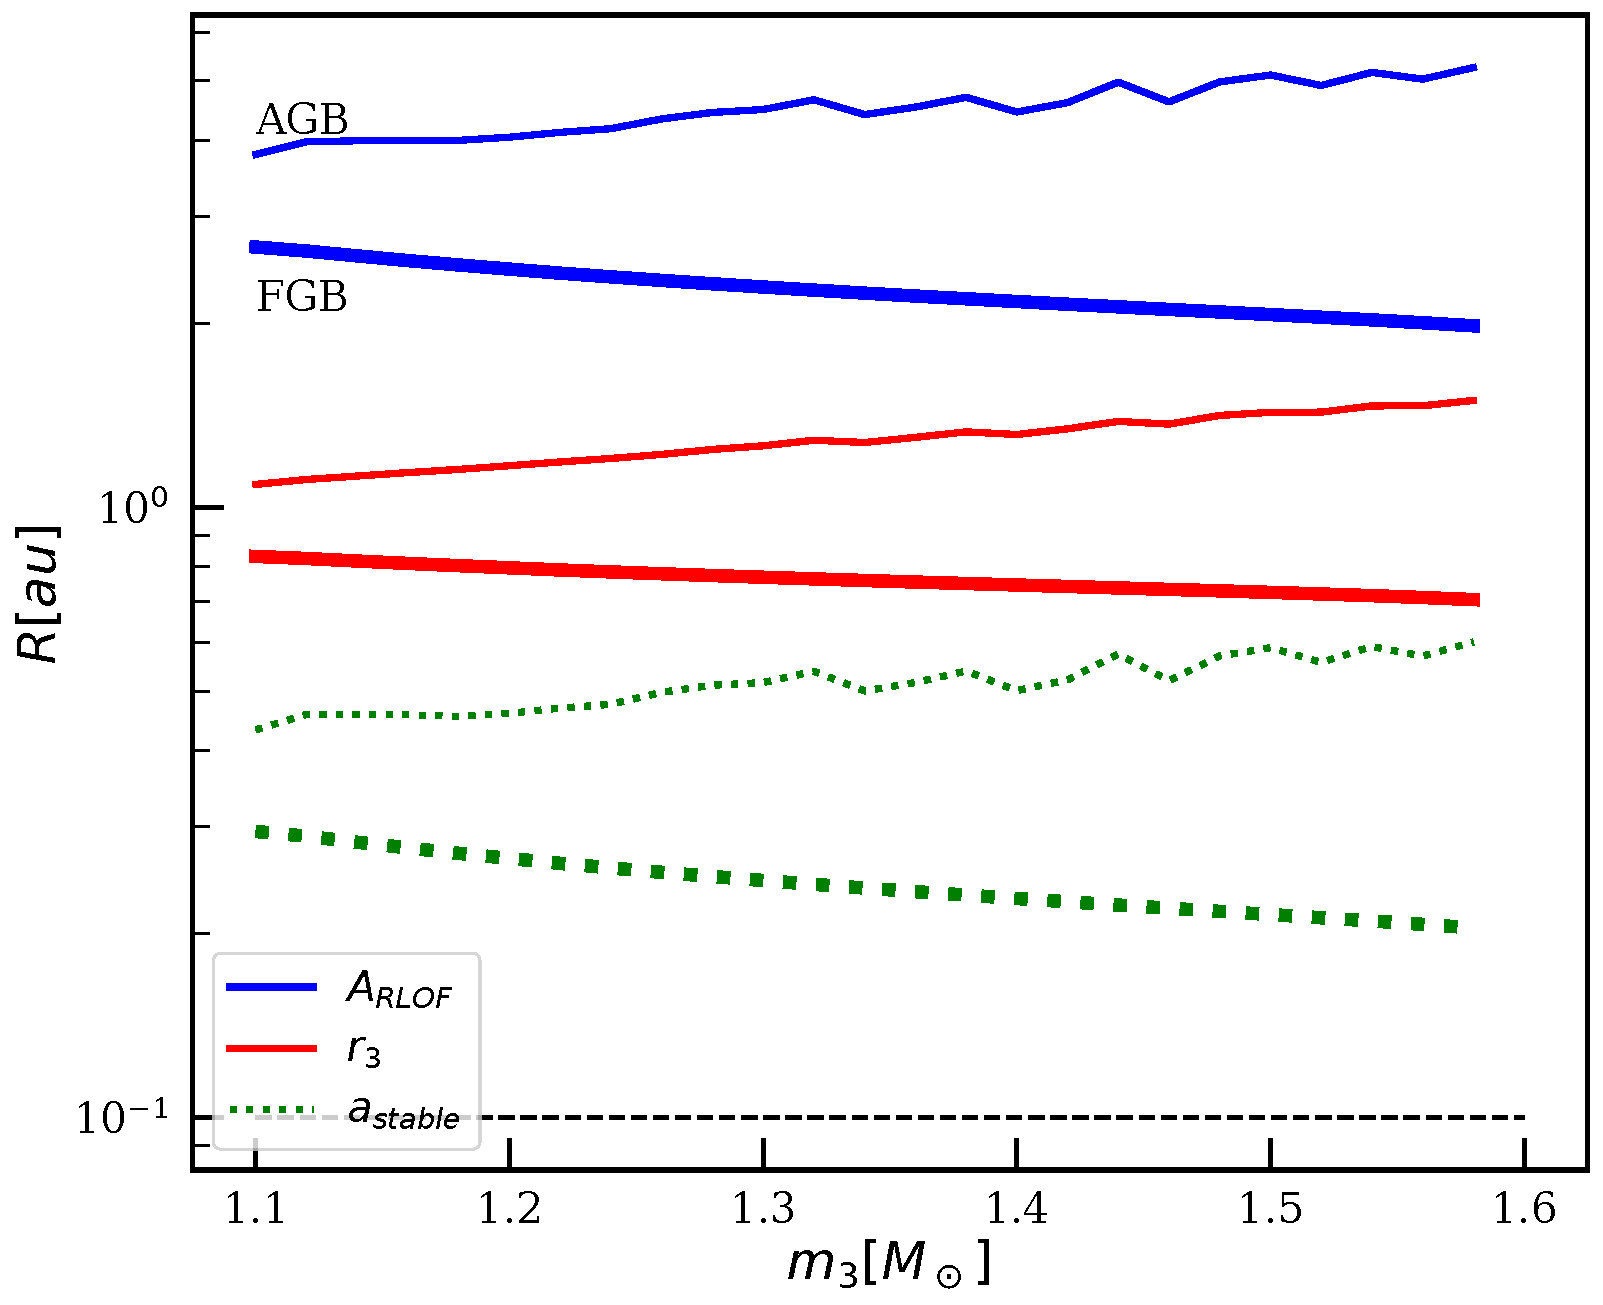
\includegraphics[width=\columnwidth]{fig_minimumstablesize.pdf}
\caption{Orbital separation as a function of the mass of the
  Roche-lobe filling outer star. The red curves gives the size at the
  first giant branch (thick curve) at the AGB (thin curve). The
  blue curve gives the orbital separation at the moment this giant fills its
  Roche-lobe assuming a circular orbit and a total inner binary mass
  of 2.0\,\MSun. The green curves give, under these conditions, the
  maximum orbital separation for a stable inner binary.
\label{fig:tertiarymass_vs_size}}
\end{figure}

In Fig.\,\ref{fig:tertiarymass_vs_size} we present..

\section{Numerical Simulations} \label{sims}

\subsection{AMUSE} \label{amuse}

We perform simulations of a triple star system of which the outer star
overfills its Roche lobe while the inner binary remains detached. The
calculations start by evolving the three stars to the same age, which
is selected such that the outer-most star fills its Roche lobe.
Constraints for the initial conditions are derived in the previous
\S\, but in \S\,\ref{Sect:ICs} we summarize the adopted initial
conditions for the simulations.

RLOF in triples using a coupled integrator to follow the complex
hydrodynamics of the mass transfer from the Roche-lobe filling outer
star to the inner binary, while keeping track of the gravitational
dynamics of the stars.  The equations of motion of the inner binary is
solved using the semi-symplectic direct N-body integrator
\texttt{Huayno} \citep{2012NewA...17..711P}. The hydrodynamics is
performed with the smoothed-particles hydrodynamics code
\texttt{Gadget2} \citep{2000ascl.soft03001S}, using an adiabatic
equation of state.  The two inner binary stars are treated as point
masses, but we allow them to accrete gas from the outer star.  This is
realized using sink-particles that co-move with the mass points in the
gravity code. While the inner two stars accrete mass, they also
accrete the appropriate amoun of angular momentum from the gas.  and
the the N-body integrator accounts of this appropriately.  For the
radius of the sink particles we adopt $10 R_\odot$ for both stars.

The N-body code as well as the hydrodynamics solver operate using
their own internal time-steps. The coupling between the two codes is
realized using the \texttt{Bridge} method in the AMUSE framework
\citep[see Sect.\.4.3.1 in][]{2013CoPhC.183..456P}.  This coupled
integrator is based on the splitting of the Hamiltonian much in the
same way as is done with two different gravity solvers by
\cite{2007PASJ...59.1095F}. With the adopted scheme, the
hydrodynamical solver is affected by the gravitational potential of
its own particles, as well as the gravitational potential of the inner
binary. The hydrodynamics, in particular the gas drag, in turn affects
the orbits of the two inner stars. With \texttt{Bridge} we realize a
second order coupling between the gravitational dynamics and the
hydrodynamics.  The interval at which the gravity and hydrodynamics
interact via \texttt{Bridge} depends on the parameters of the system
we study, but typically we achieve converged solutions when this time
step is about a fraction of 1/100 of the inner binary orbital period.

\subsection{Initial Conditions} \label{Sect:ICs}

We adopt initial component masses of m$_{\rm 1}$ = 1.1 M$_{\rm \odot}$
and m$_{\rm 2}$ = 0.9 M$_{\rm \odot}$ for the inner binary components,
and m$_{\rm 3}$ = 1.2 M$_{\rm \odot}$ for the tertiary star.  We
evolved the 1.2\,\MSun\, star using the MESA stellar evolution code
\cite{2011ApJS..192....3P} to a radius of about 255\,\RSun.  By this
time the star has lost 0.13\,\MSun\, in a stellar wind.  With these
parmeters the orbital separation of the outer binary becomes 3.86\,au,
and the mass loss has driven a slight eccentricity from initiall
circular orbit to about 0.0082 at the moment of Roche-lobe
overflow. We chose a relative initial inclination of $i = 9^\circ$
between the inner and the outer orbit.

In fig.\,\ref{fig:topview_at_t0} we present a top view of the triple
system at the onset of Roche-lobe overlofw.  

\begin{figure}[ht!]
  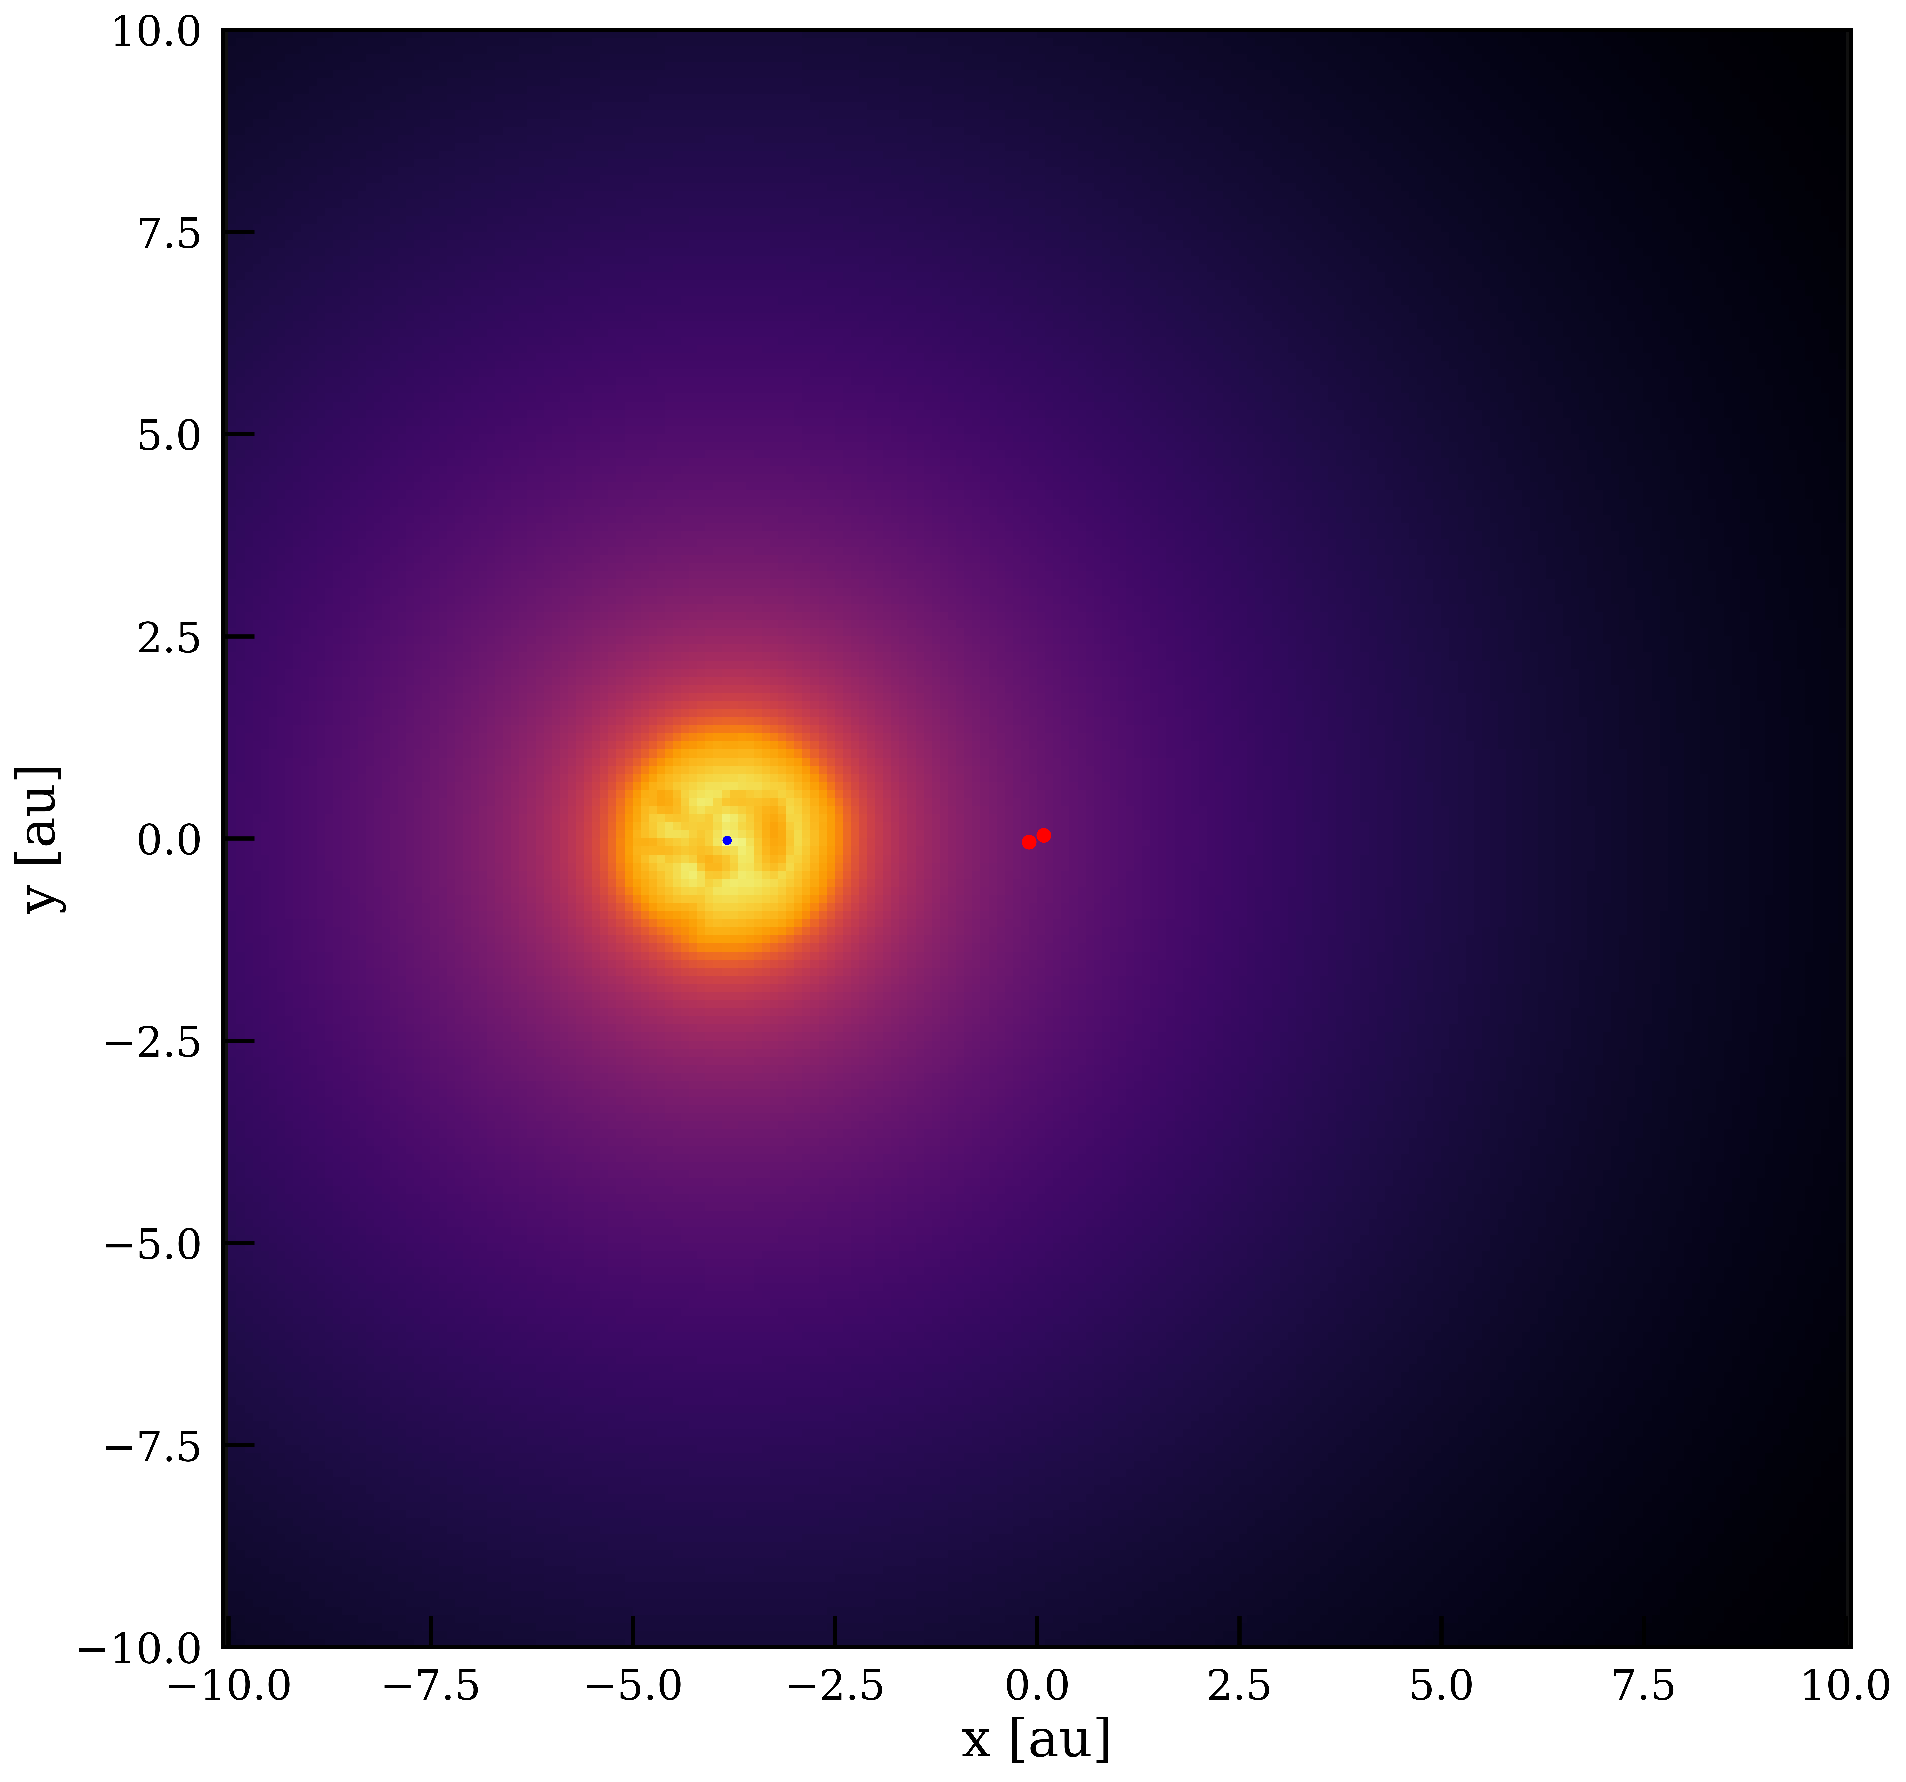
\includegraphics[width=\columnwidth]{fig_t0_N80000_M012MSun1109MSun_a02au_e00_inc9deg.pdf}
\caption{top view of the triple system in which the outer star
  (represented by 80000\,sph particles and a core particle of
  0.4\,\MSun (blue bullet). The two companion stars are represented as
  red bullets (to the right).
\label{fig:topview_at_t0}}
\end{figure}

\section{Results} \label{results}

In fig.\,\ref{fig:topview_at_t1000day} we show the same triple at
after 1000\,days of evolution.

\begin{figure}[ht!]
  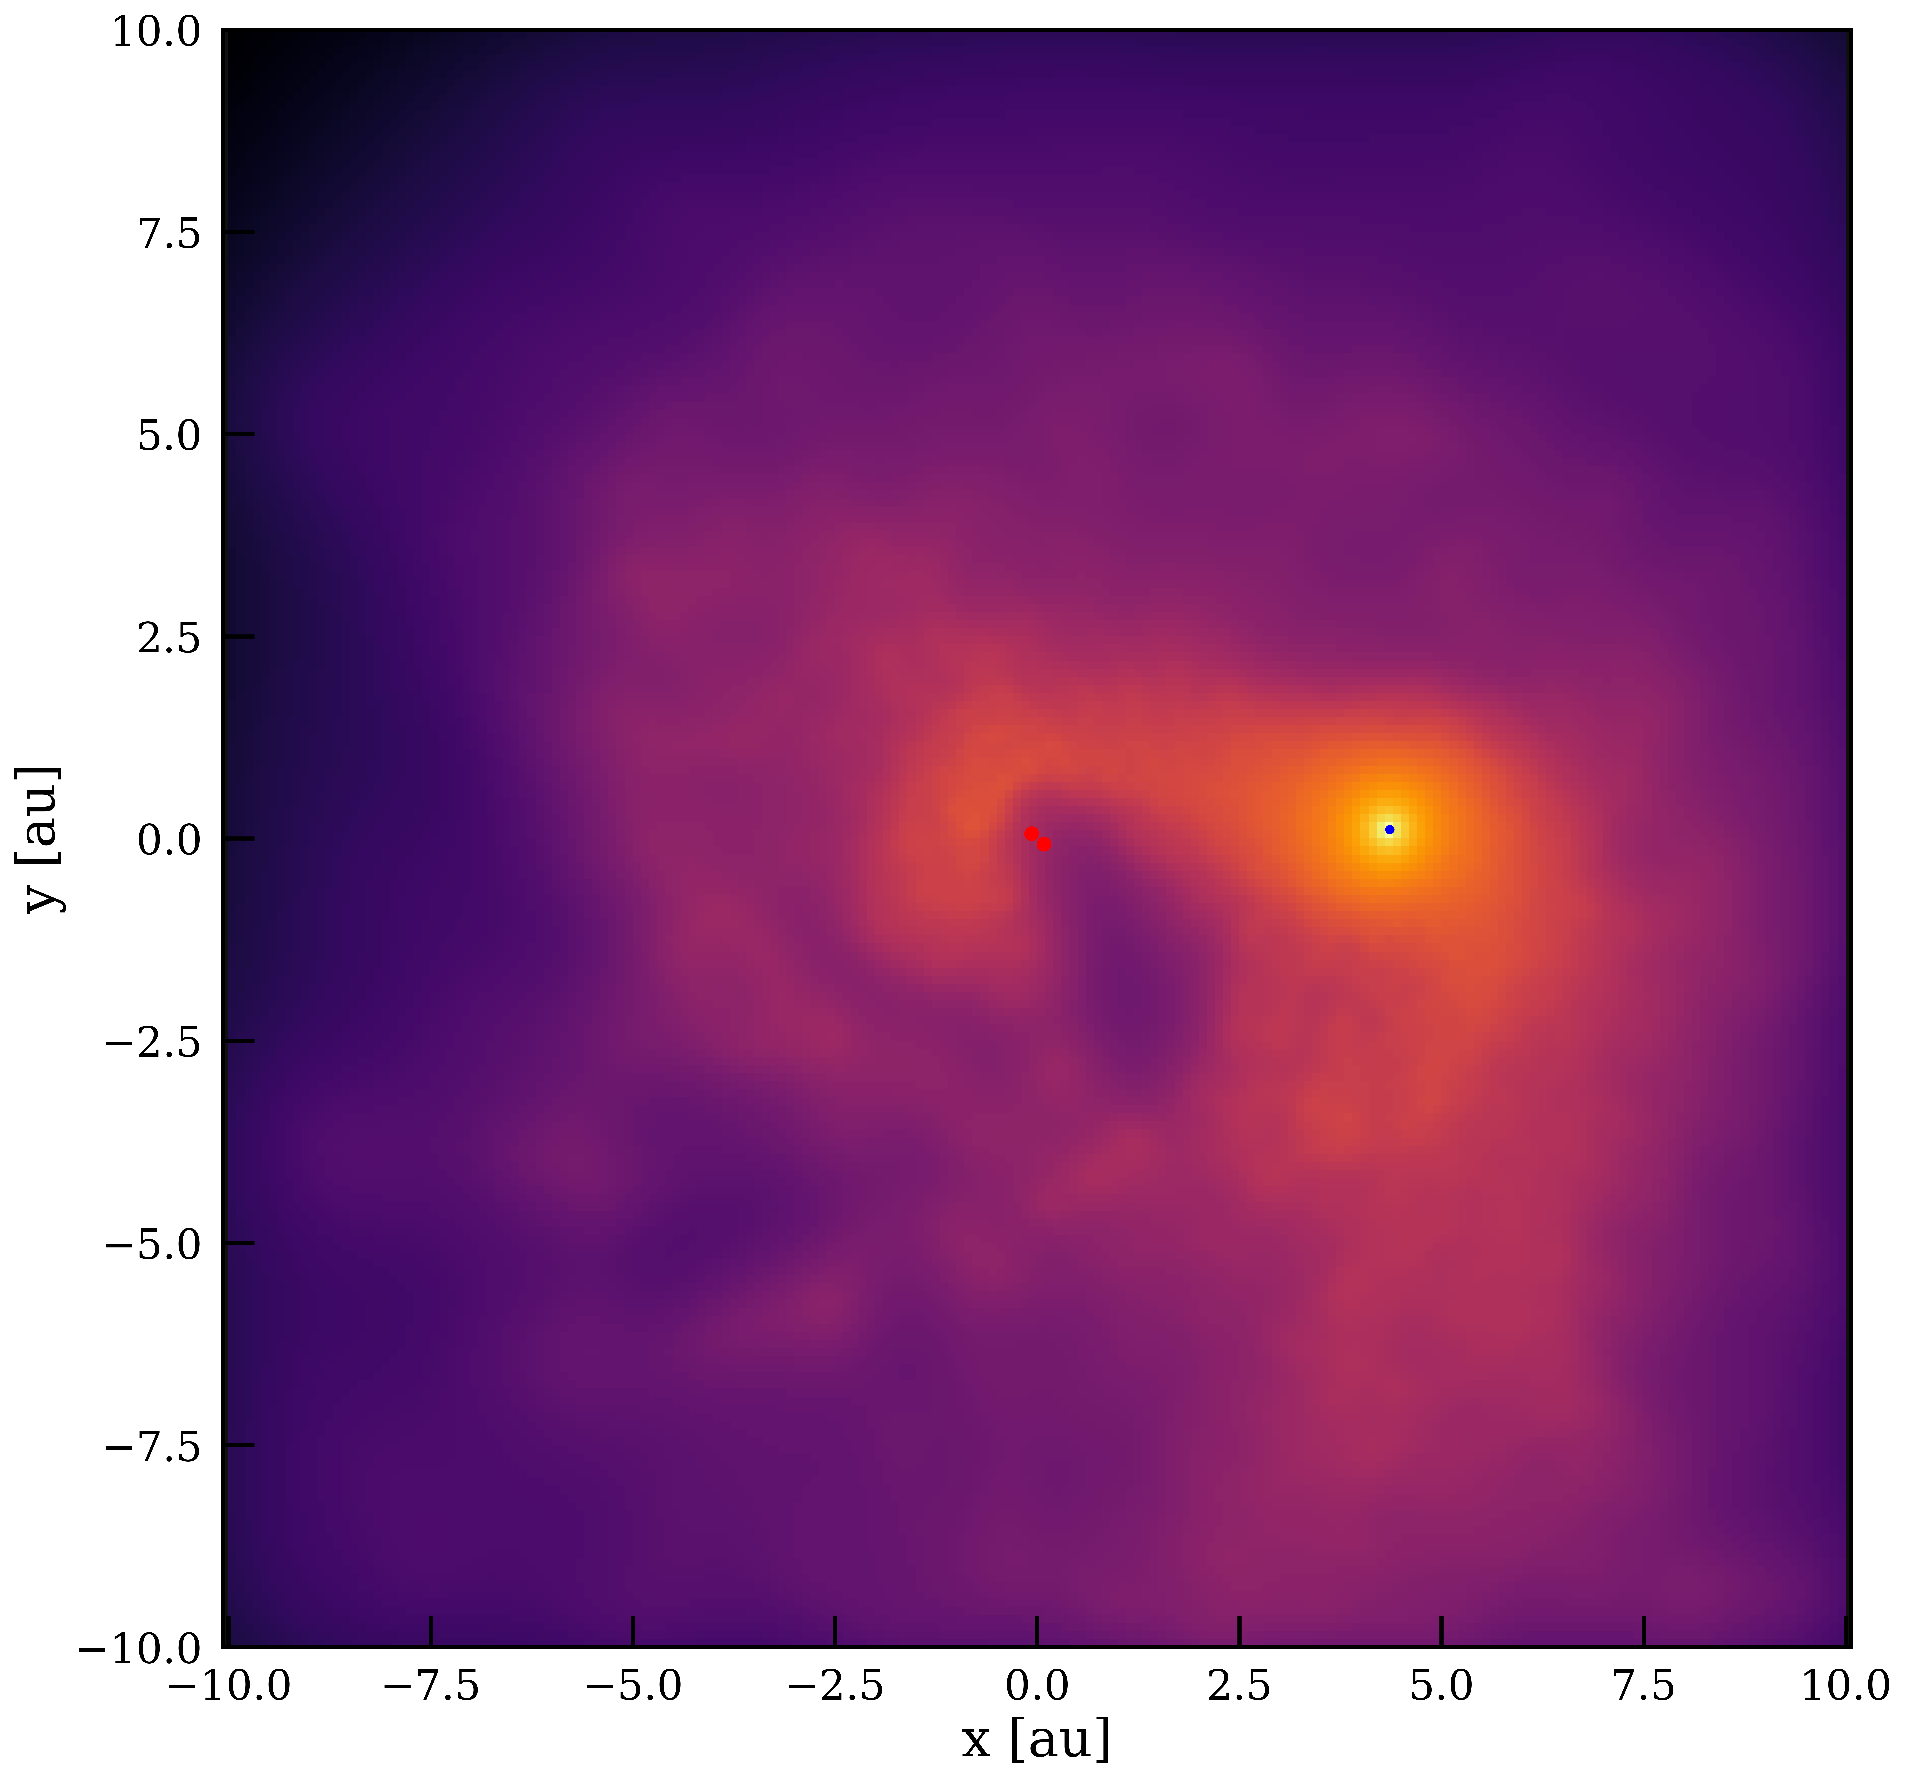
\includegraphics[width=\columnwidth]{fig_t600_N80000_M012MSun1109MSun_a02au_e00_inc9deg.pdf}
\caption{Same as Fig.\,\ref{fig:topview_at_t0} but at an age of $t
  \simeq 996days$.
\label{fig:topview_at_t1000day}}
\end{figure}

In fig.\,\ref{fig:mass_evolution_for_M1.2M1.1M0.9a02e00i09}

\begin{figure}[ht!]
  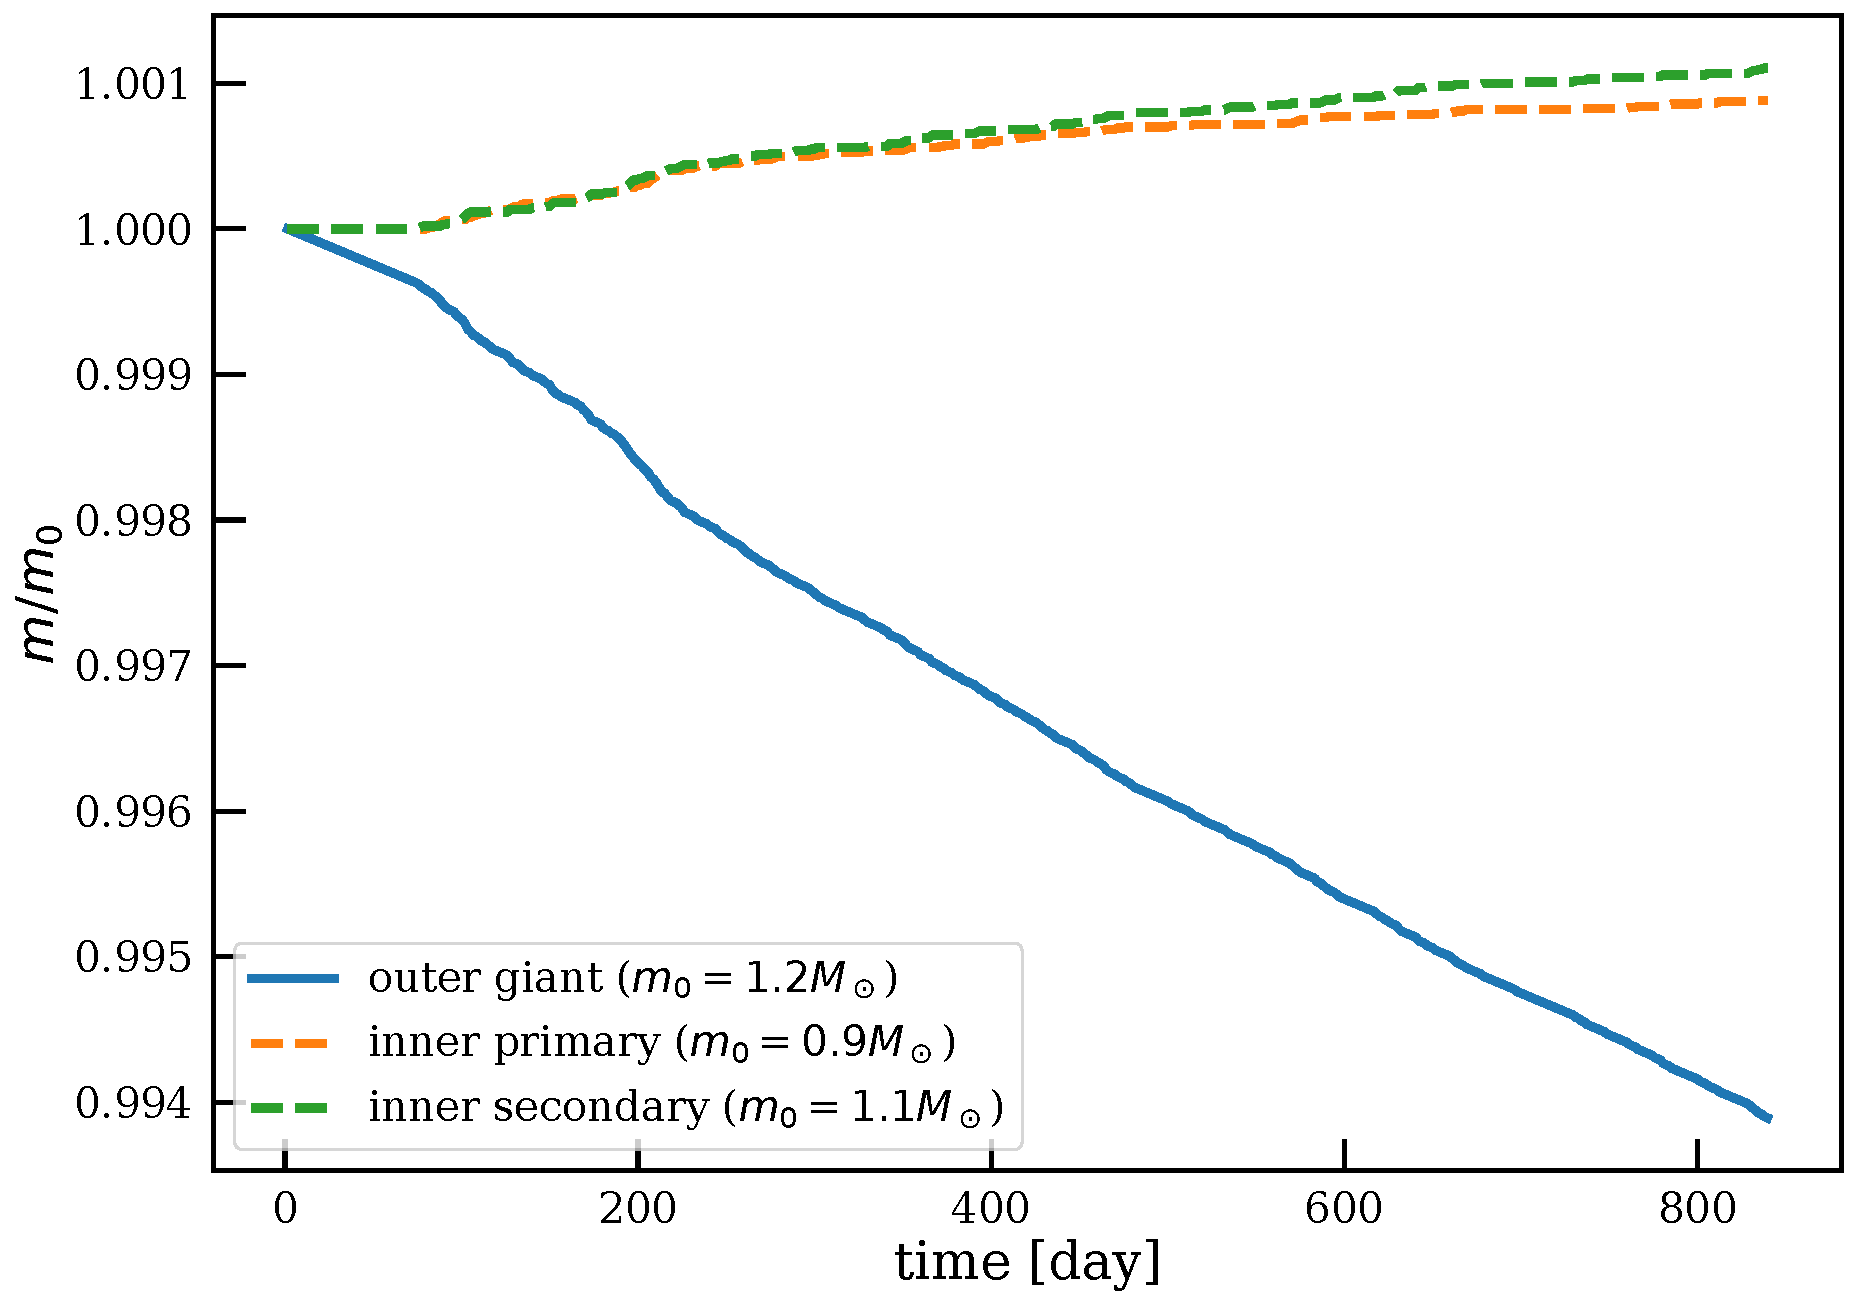
\includegraphics[width=\columnwidth]{fig_MvsTime_N80k_M012R100RSun1109MSun_a02au.pdf}
\caption{Evolution of the masses (normalized to those at the moment of
  Roche-lobe overflow) of each of the three stars as a function of
  time for the first 1000\,days. (see Fig.\,\ref{fig:topview_at_t0}
  for a face-on representation of the initial conditions and
  fig.\,\ref{fig:topview_at_t1000day} for the final conditions}.  The
green and orange dashed curves give the masses of the inner two stars,
whereas the solid blue curve is the mass of the outer most star.
\label{fig:mass_evolution_for_M1.2M1.1M0.9a02e00i09}
\end{figure}


\section{Summary and Discussion} \label{discussion}



This
choice for the initial mass of the outer tertiary is critical since it
ensures that the donor star during the mass transfer process will have
a radiative envelope \citep[e.g.][]{maeder09}.  In turn, this ensures
that the mass transfer will be maximally conservative, such that the
accretion stream will be maximally stable, accreting at a stable and
constant rate \citep[e.g.][]{iben91}.

In this Letter, we have proposed a formation scenario for double BS equal-mass compact binaries, as observed for Binary 7782 in the old open cluster NGC 188.  The proposed scenario involves mass transfer from an evolved outer tertiary companion, which is accreted by the inner binary via a circumbinary disk.  Our scenario makes several predictions for the observed properties of a hypothetical outer triple companion, now a WD.  These are:

\begin{enumerate}

\item For the predicted outer tertiary orbit, the present-day semi-major axis should lie between 220 days $\lesssim$ P$_{\rm out}$ $\lesssim$ 1100 days, assuming initial masses for the inner binary components of m$_{\rm 1} =$ 1.1 M$_{\odot}$ and m$_{\rm 2} =$ 0.9 M$_{\odot}$ and an outer tertiary mass of m$_{\rm 3} =$ 1.4 M$_{\odot}$.

\item Larger final WD masses, and hence core masses for the donor at the time of mass transfer, should correspond to larger final outer orbital periods for the tertiary.  This is because the Roche radius is larger for larger outer orbital periods, such that the donor must evolve to larger radii, and hence core masses, before the onset of mass transfer.

\item For the inner binary, the rotational axes of the BSs should be aligned with each other and the orbital plane of the outer tertiary WD.  This is because accretion onto the BS progenitors proceeds via an accretion disk, that forms at the circularization radius and that has an orbital plane aligned with that of the outer tertiary.

\item The BSs in the inner binary should have roughly equal masses, independent of their initial masses.  This is because it is the lowest mass object that typically accretes the fastest, since its orbital velocity and distance relative to the circumbinary disk is typically the lowest \citep[e.g.][]{haiman09,farris15,rafikov16,kelley17}.  This quickly brings the mass ratio toward unity.  This predicts that the initially lower mass MS star should accrete the most, and should hence be polluted more significantly by any accreted material.  This could be observable in the surface layers of a radiative star.  If the donor is an RGB star, the accretor will be enriched in mostly carbon, oxygen and helium.  If the donor is an AGB star, it will be enriched in mostly s-process elements.

\item Twin BSs in compact binaries formed from the proposed mechanism should be more frequent in younger clusters with ages $\lesssim$ 4-6 Gyr.  This is because clusters with a main-sequence turn-off mass $\lesssim$ 1.2 M$_{\odot}$ have convective envelopes \citep[e.g.][]{iben91,maedoer09}, and a radiative envelope for the donor in a mass transferring binary ensures stable accretion on to the accretor.

WHAT ELSE?  SOMETHING RELATED TO TIMESCALES AND THE PROBABiLitY OF OBSERVING THE WD?

\end{enumerate}

Finally, in future work, we intend to explore the implications of the mechanism proposed here for other types of stellar triples.  The results highlight that specific theoretical predictions can often be made.  For example, if two white dwarfs form the inner compact binary, than circumbinary accretion could push one of them above the Chandrasekhar mass limit.  Upon explosion, its WD companion would be ejected at roughly the orbital velocity at the time of explosion, producing a hypervelocity WD.  This predicts hot hypervelocity WDs with masses very close to the Chandrasekhar mass limit for this scenario.  Similarly, if the two WDs are replaced with two neutron stars (NSs), then one NS will likely accrete to surpass the critical supernova limit, upon which time it explodes to become a black hole and receives a strong natal kick.  The NS companion would have a very comparable mass to the newly formed black hole progenitor at the time of explosion, and could potentially be used to constrain the maximum NS mass.  More work needs to be done here to evaluate whether or not there is any parameter space for the products of this scenario that will allow for a mass determination for the original NS companion in the putative compact NS-NS binary.

\acknowledgments

N.W.C.L. acknowledges support from a Kalbfleisch Fellowship at the
American Museum of Natural History.  SPZ would like to thank Norm
Murray and CITA for their hospitality during my long-term visit.

\bibliographystyle{apj}
\bibliography{BBS7782}


%\input /home/spz/Latex/lib/bib/references
%\bibliographystyle{/home/spz/Latex/lib/styles/elsevier/elsarticle-num} 
%\bibliography{references}      


\end{document}
